\documentclass[12pt]{article}
\usepackage[utf8]{inputenc}
\usepackage[T1]{fontenc}
\usepackage[french]{babel}
\usepackage{graphicx}
\usepackage{amsmath}
\usepackage{amssymb}
\usepackage{hyperref}
\usepackage{eso-pic}
\usepackage{listings}
\usepackage[export]{adjustbox}
\usepackage{multicol}
\usepackage[font=small,labelfont=bf]{caption}
\usepackage[linesnumbered,ruled,french,onelanguage]{algorithm 2e}
\usepackage{tikz}


\makeatletter
\makeatother


\newcommand{\HRule}{\rule{\linewidth}{0.5mm}}
\newcommand{\blap}[1]{\vbox to 0pt{#1\vss}}
\newcommand\AtUpperRightCorner[3]{%
  \put(\LenToUnit{\dimexpr\paperwidth-#1},\LenToUnit{\dimexpr\paperheight-#2}){\blap{\llap{#3}}}%
   }

     \title{\LARGE{Analyseur de livre dont vous êtes le héros}
   }  
   
\author{
\begin{center}
\textsc{KAMGANG KENMOE} Miguel Jordan \\
\textsc{Dioukou} Moussa Sissoko \\
\textsc{ABOGOUNRIN} Ayath \\
\textsc{Alhazzaa} Laith \\
\end{center}
}

\date{\today}
\makeatletter
 
\begin{document}
 
\begin{titlepage}
   
    \AddToShipoutPicture{
        \AtUpperRightCorner{1.5cm}{1cm}{
\includegraphics[width=6.5cm]{images/logo.png}}
    }
 
  \begin{center}
     \vspace*{4cm}
     \textsc{\@title}
     \HRule
     \vspace*{0.5cm}
     \large{\@author}
 \end{center}
    
 \begin{center}
    \vspace*{0.5cm}
    \large{\@date} 
 \end{center}
    
 \begin{center}svn checkout https://forge.info.unicaen.fr/svn/analyseur-de-livre 
    \vspace*{0.5cm}
    Chargée du TP :  CAGNIOT Emmanuel
  \end{center}
    
  \begin{center}
    \vspace*{0.5cm}
    Groupe :  2B
  \end{center}
 
  \vspace*{4.2cm}
 
  \begin{center}
     Année universitaire 2023-2024
  \end{center}
 
\end{titlepage}svn checkout https://forge.info.unicaen.fr/svn/analyseur-de-livre 
\ClearShipoutPicture

\newpage
	
\tableofcontents

\newpage

\section{Introduction}
 L’unité d’enseignement Projet 1 a pour objectif de nous faire comprendre le concept de la programmation orientée objet, nous initiés aux implémentations des algorithmes  et parfaire notre maitrise de java. \\ Pour cela des groupes de 4 étudiants ont été formés et plusieurs projets ont été proposés, comme Interpréteur de systèmes de Lindenmeyer, Simulateur de jeux de la vie, Analyseur de livres dont vous êtes le héros, Générateur de castors affairés, etc. Parmi ceux ci notre groupe a choisi Analyseur de livres dont vous êtes le héros. À travers ce rapport, nous allons explorer les principaux aspects du jeu, y compris son concept.

\subsection{Présentation du projet}

\textbf{C'est quoi le livre dont vous êtes le héros?}
\newline
\newline
   Le livre dont vous êtes le héros(ou LDVEH) est un jeu qu'il faut jouer en solitaire. Il consiste à choisir un livre, la narration de ce dernier est décomposées en paragraphes, dispersés dans le livre. Des liens, en fonction des choix du lecteur, permettent d’aller d’un paragraphe à l’autre. Ainsi, un LDVEH peut être représenté par un graphe, permettant de naviguer à travers le livre en utilisant des choix interactifs.

\textbf{C'est quoi l'Analyseur de livre dont vous êtes le héros?}
\newline
\newline
  Analyseur de livre dont vous êtes le héros est le fait de choisir un livre dont vous êtes le héros déjà existant et d'effectuer différents analyse possible sur le livre. Donc différents analyse sur le graphe, il serait donc intéressant de produire des réponses à des questions du type :  Quel est le chemin le plus court qui mène a la défaite?, Quel est le plus long chemin?, Quelle est la probabilité de victoire après une marche aléatoire?, Quel est le nombre de combat dans le livre?,quelle est la difficulté du livre? etc.
  
\subsection{Objectif du projet}

  Le but de ce projet est de développer un programme permettant de faire différents analyses sur un graphe. Dans un premier temps il s'agira d'afficher un graphe à l'aide d'un algorithme de force. Dans un second temps, il s'agira d’implémenter différents algorithmes afin de répondre aux différents questions qu'on peut poser sur le graphe.Comme supplément nous pouvons étendre notre modèle du graphe en parlant combats dans les livre. 

\section{L'analyse du projet}

\subsection{Diagramme de classe}
  Pour atteindre nos objectifs nous avons divisés le projet en 05 packages à savoir:
  
\vspace{12pt plus 5pt minus 5pt}

\textbf{backbone :} Il contient les classes Book et Page qui représente le cœur de notre jeu
\vspace{12pt plus 5pt minus 5pt}

\textbf{extraction :} Dans ce package se trouve toutes les classes qui nous ont permis d'extraire les pages de notre livre à partir d'un fichier Json ou d'un fichier Texte

\vspace{12pt plus 5pt minus 5pt}

\textbf{model :} Il contient toutes les classes utilisées comme modèle du jeu, nous avons la classe Node qui représente les nœuds dans notre graphe donc chaque page du livre, la classe Edge représente l'arête entre deux Nodes c'est à dire le chemin pour passer d'une page à une autre et enfin la classe Graph qui représente notre graphe.

\vspace{12pt plus 5pt minus 5pt}

\textbf{questions :} Ce package ne contient rien d'autre que les différents analyses qu'on peut faire sur notre graphe, à savoir: le plus court chemin,le plus long chemin, tous les pages contenant les combats, tous les pages de défaite et la probabilité de victoire après une marche aléatoire.

\vspace{12pt plus 5pt minus 5pt}

\textbf{view :} Dans ce package se trouve toutes les classes de la Vue. On a la classe Fruchterman-Reingold qui n'est rien d'autre que l'algorithme de force utilisé pour la visualisation du graphe,nous avons aussi les classes GraphVisualization, GUI et le Main qui nous permet d'afficher notre graphe.

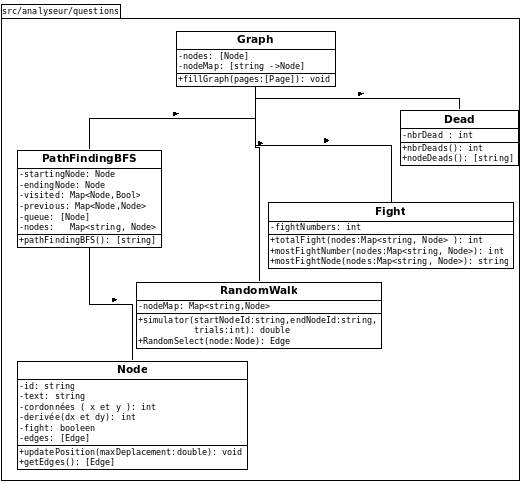
\includegraphics[width=15 cm,height=15cm]{images/Diagramme1.png}

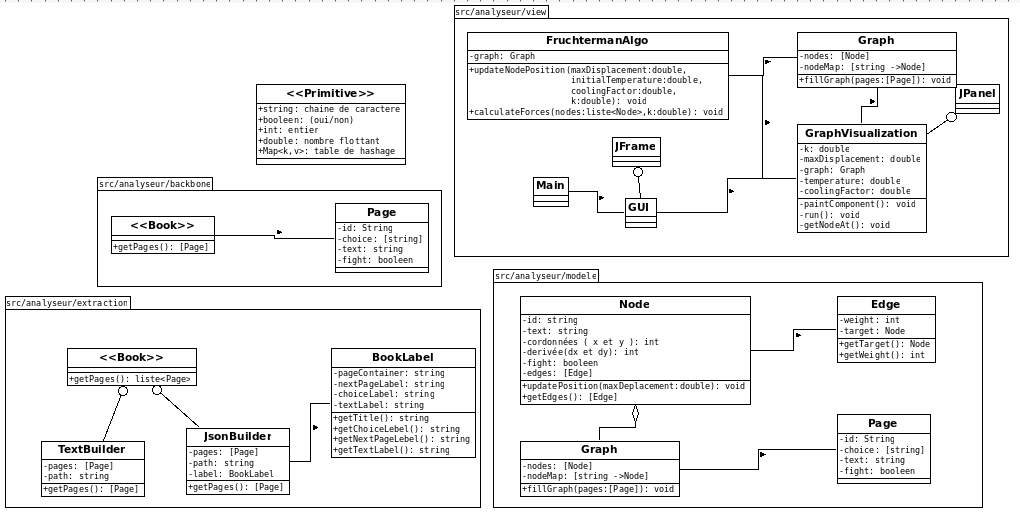
\includegraphics[width=17cm,height=16cm]{images/Diagramme2.png}
 
\section{Les différents étapes du projet}
	Dans un premier temps, nous avons commencé par créer nos classes Page et Book.
La classe Page représente les pages dans notre livre, on peut aussi dire les nœuds de notre graphe et la classe Book n'est rien d'autre que l'ensemble des pages, donc le livre à analyser.

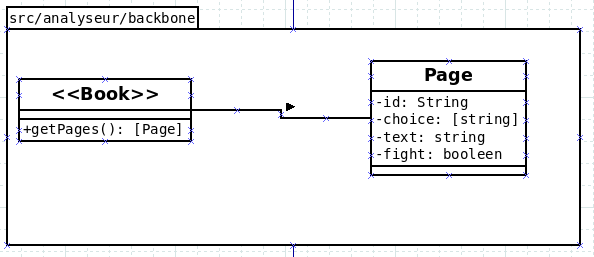
\includegraphics[width=10cm,height=8cm]{images/BookPage.png} 	

 \subsection{Extraction des pages}
 \begin{itemize}
 \item Fichier text :
 Permet d'extraire les données via un fichier texte en utilisant les expressions régulières
 \item Fichier Json :
 Permet d'extraire les données via un fichier Json en utilisant la librairie Javax.json
 
 \end{itemize}
 
 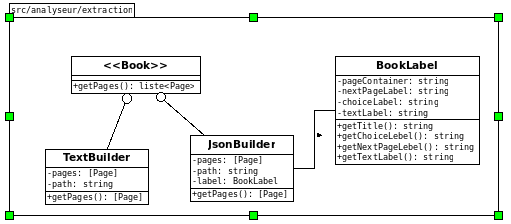
\includegraphics[width=10cm,height=8cm]{images/extraction.png} 	

 
 \subsection{Visualisation du graphe}

   Comme on l'avait dit on peut représenter le jeu LDVEH par un graphe. Pour la visualisation de notre graphe nous avons découvrir plusieurs algorithmes de forces tels que l'algorithme de Harel et Koren, algorithme de Kamada et Kawai, algorithme de Fruchterman-Reingold , etc.
   
\vspace{12pt plus 5pt minus 5pt}

Pourquoi choisi l'algorithme de Fruchterman-Reingold ? \newline

   En raison de la capacité de ce dernier à produire des dispositions spatiales efficaces et esthétiquement agréable des arêtes et des nœuds. Il faut aussi dire que l'algorithme de Fruchterman-Reingold  est facile à comprendre du point de vue de son code , non seulement ça il est bien documenté et à été également bien étudié. 
\vspace{12pt plus 5pt minus 5pt}

C'est quoi l'algorithme de Fruchterman-Reingold ? \newline

   L'algorithme de Fruchterman-Reingold est un algorithme de disposition de graphe utilisé pour visualiser des graphes de manière à ce que les nœuds soient répartis de manière équilibrée et à ce que les arêtes ne se croisent pas autant que possible. Il a été proposé par Thomas Fruchterman et Edward Reingold en 1991. 
Il est basé sur un modèle de stimulation physique dans lequel les nœuds se repoussent les uns les autres tandis que les arêtes qui sont considérés comme des ressorts, exercent une force d'attraction sur les nœuds qu'elles relient, permettant ainsi de trouver un équilibre entre la séparation des nœuds et la clarté des arêtes.

\vspace{12pt plus 5pt minus 5pt}

Algorithme de Fruchterman-Reingold  \newline

\begin{algorithm}[H]
  \SetAlgoLined
  \KwData{Width $W$, Length $L$, Graph $G = (V, E)$, Constant $p$, Initial temperature $t$, Number of iterations}
  \KwResult{Adjusted positions of vertices}

  $area \leftarrow W \times L$\;
  $k \leftarrow p$\;
  $areaPerVertex \leftarrow \frac{area}{|V|}$\;
  Initialize positions of vertices randomly\;
  \While{not reached maximum iterations}{
    \ForEach{vertex $v \in V$}{
      Calculate repulsive forces\;
      $v.disp \leftarrow 0$\;
      \ForEach{vertex $u \in V$}{
        \If{$u \neq v$}{
          $\delta \leftarrow v.pos - u.pos$\;
          $v.disp \leftarrow v.disp + \left(\frac{\delta}{|\delta|}\right) \times fr(|\delta|)$\;
        }
      }
    }
    \ForEach{edge $e \in E$}{
      Calculate attractive forces\;
      $\delta \leftarrow e.v.pos - e.u.pos$\;
      $e.v.disp \leftarrow e.v.disp - \left(\frac{\delta}{|\delta|}\right) \times fa(|\delta|)$\;
      $e.u.disp \leftarrow e.u.disp + \left(\frac{\delta}{|\delta|}\right) \times fa(|\delta|)$\;
    }
    \ForEach{vertex $v \in V$}{
      Limit displacement and prevent from going outside the frame\;
      $v.pos \leftarrow v.pos + \left(\frac{v.disp}{|v.disp|}\right) \times \min(v.disp, t)$\;
      $v.pos.x \leftarrow \min\left(\frac{W}{2}, \max\left(-\frac{W}{2}, v.pos.x\right)\right)$\;
      $v.pos.y \leftarrow \min\left(\frac{L}{2}, \max\left(-\frac{L}{2}, v.pos.y\right)\right)$\;
    }
    Cool down the temperature $t$\;
  }
  \caption{Force-Directed Graph La Fruchterman-Reingold  \newline
yout Algorithm}
\end{algorithm}


Pour afficher notre graphe, nous avons fait recours à l'interface graphique, d'où la création des classes GraphVisualization et GUI.

Dans la classe GraphVisualization, nous avons utiliser JPanel comme conteneur, ce qui nous a permis de représenter nos nœuds, leurs dispositions aléatoire dans la fenêtre, nos arêtes ainsi que les différents actions que peut effectuer la souris sur les nœuds.

GUI est une classe qui hérite de JFrame, nous l'avons utiliser pour avoir une fenêtre dans laquelle on a placé le JPanel.

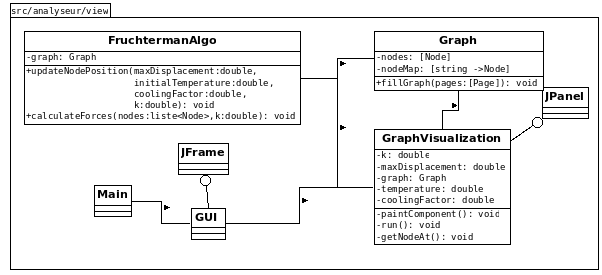
\includegraphics[width=12cm,height=12cm]{images/view.png}


 \subsection{Les analyses sur le graphe}
   \begin{itemize}
   \item Le plus court chemin \newline
  Afin de trouver le plus court chemin pour atteindre une page ou la mort, nous avons trouver plusieurs algorithmes, nous pouvons citer: algorithme de Dijkstra,algorithme de Bellman-Ford, algorithme Breadth-First Search(BFS).
  Nous avons choisi l'algorithme de Breadth-First Search pour sa simplicité et sa rapidité , non seulement ça les poids de nos arêtes sont égaux et le graphe n'a pas de pondération négative, il est donc parfait pour nous d’utiliser BFS pour la recherche du plus court chemin sans avoir à faire assez de calcul.
 
   \item Tous les pages contenant les combats \newline
Afin de trouver tous pages contenant les combats, nous essayer d'extraire tous les synonymes de combats, et tant qu'il y a un synonyme dans la page, on déduit que la page contient de combat, puis on l'affiche.
   \item Tous les nœuds de défaite \newline
Dans cette classe pour trouver tous les nœuds de défaite, on a pensé au nœuds qui n'ont pas de successeur, il suffit d'arriver sur ces nœuds pour atteindre la mort, donc ne plus avoir de chemin possible pour continuer. Nous avons donc afficher le nombre de ces nœuds et ensuite les afficher.

 \item La  probabilité de victoire après une marche aléatoire \newline
 \item Le plus long chemin \newline
   
 
 \end{itemize}
 
 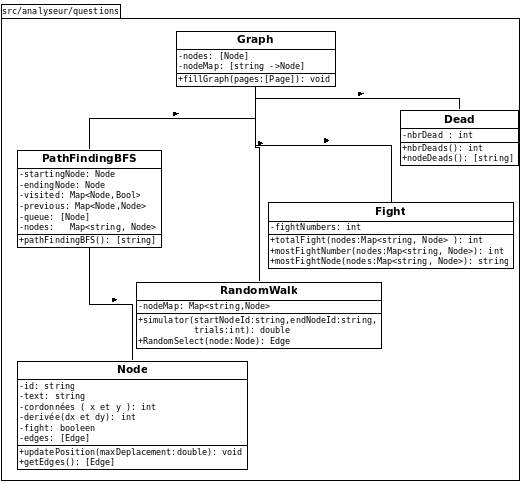
\includegraphics[width=12cm,height=12cm]{images/Diagramme1.png}

 
\section{Le rendu final de notre graphe}
Pour lancer le jeu en version graphique rendez-vous dans la racine du projet,ouvrez un
terminale et taper les commandes suivantes :

\begin{itemize}
 \item \textbf{ant compile}
 \item \textbf{ant runMain}
 
\end{itemize}


Une fois le jeu lancé vous tomberez sur la fenêtre principale ci dessous
   
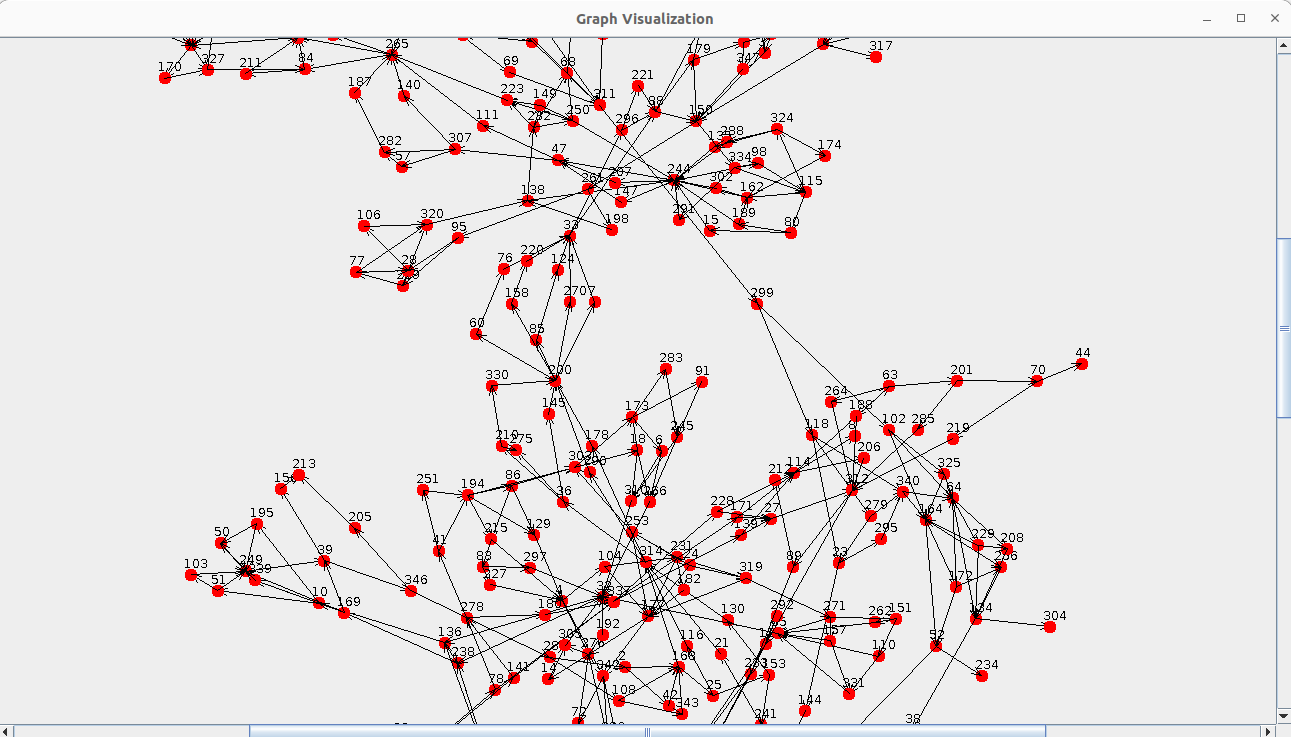
\includegraphics[width=16cm,height=16cm]{images/rendu.png}

\vspace{12pt plus 5pt minus 5pt}

En faisant un clique droit sur la souris on peut visualiser les paragraphes

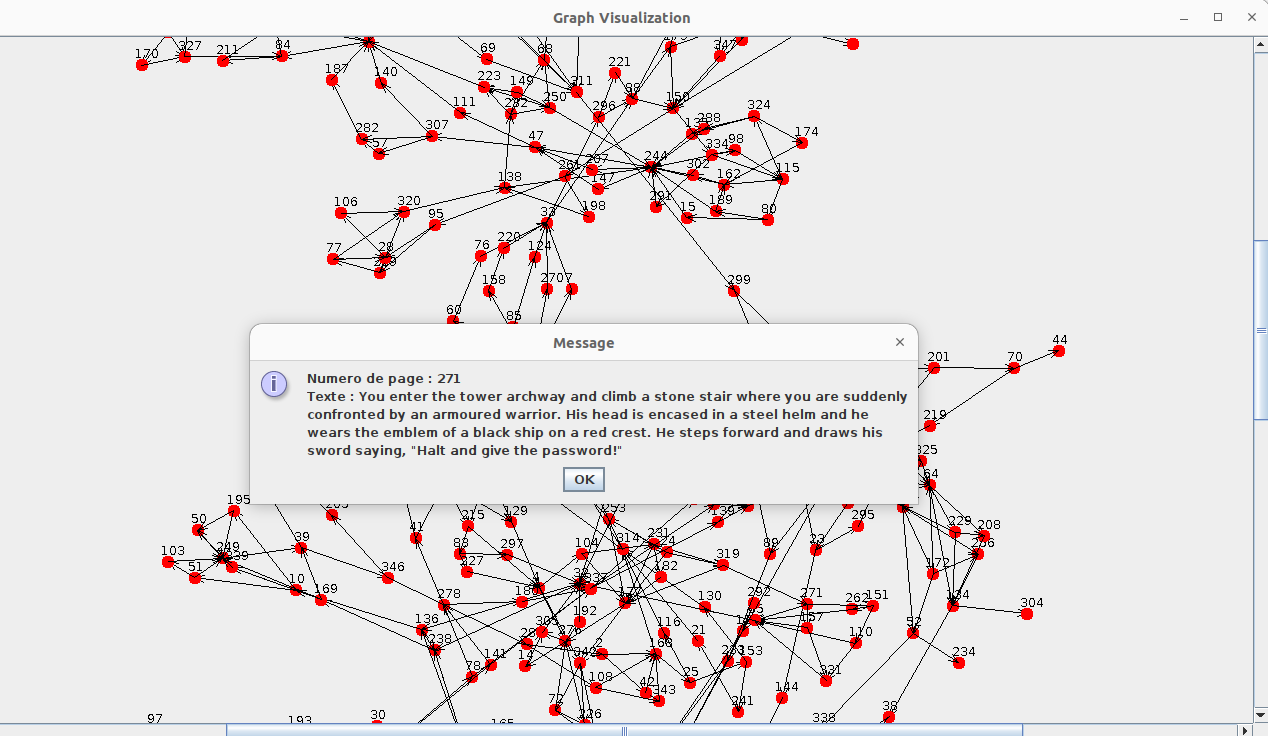
\includegraphics[width=16cm,height=16cm]{images/rendu2.png}

\vspace{12pt plus 5pt minus 5pt}

Pour afficher les différentes pages du fichier Text

\begin{itemize}
 \item \textbf{ant compile}
 \item \textbf{ant runText}
 
\end{itemize}

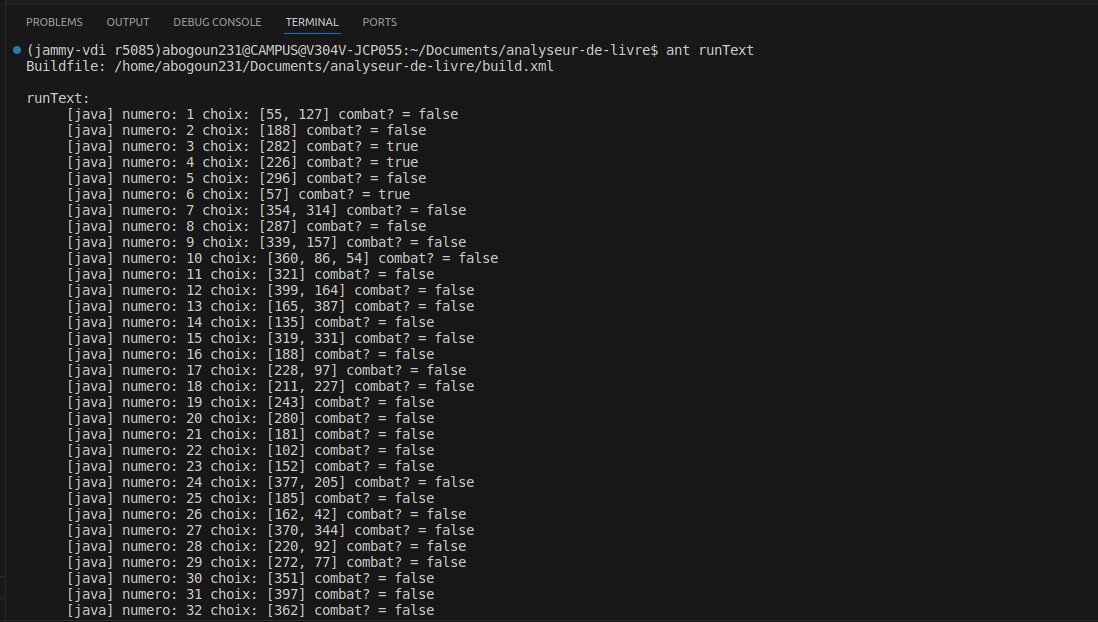
\includegraphics[width=16cm,height=16cm]{images/text.png}

Pour afficher les différentes pages du fichier Json

\begin{itemize}
 \item \textbf{ant compile}
 \item \textbf{ant runJson}
 
\end{itemize}
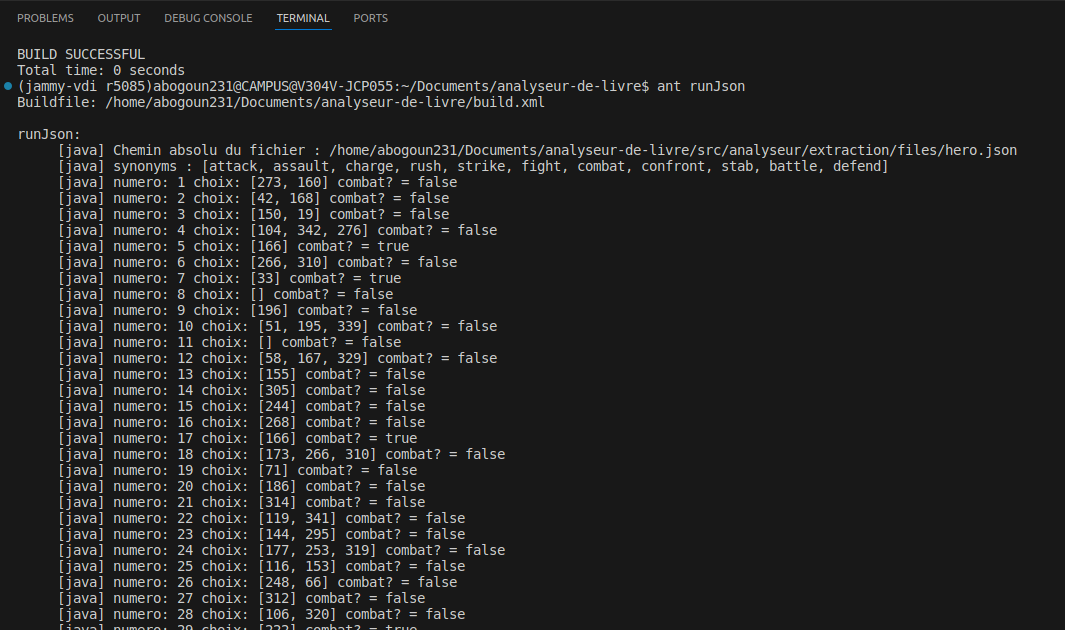
\includegraphics[width=16cm,height=16cm]{images/json.png}

Nous avons une classe MainAnalyse pour afficher les différents analyses qu'on a effectué sur le graphe

\begin{itemize}
 \item \textbf{ant compile}
 \item \textbf{ant runMainAnalyse}
 
\end{itemize}
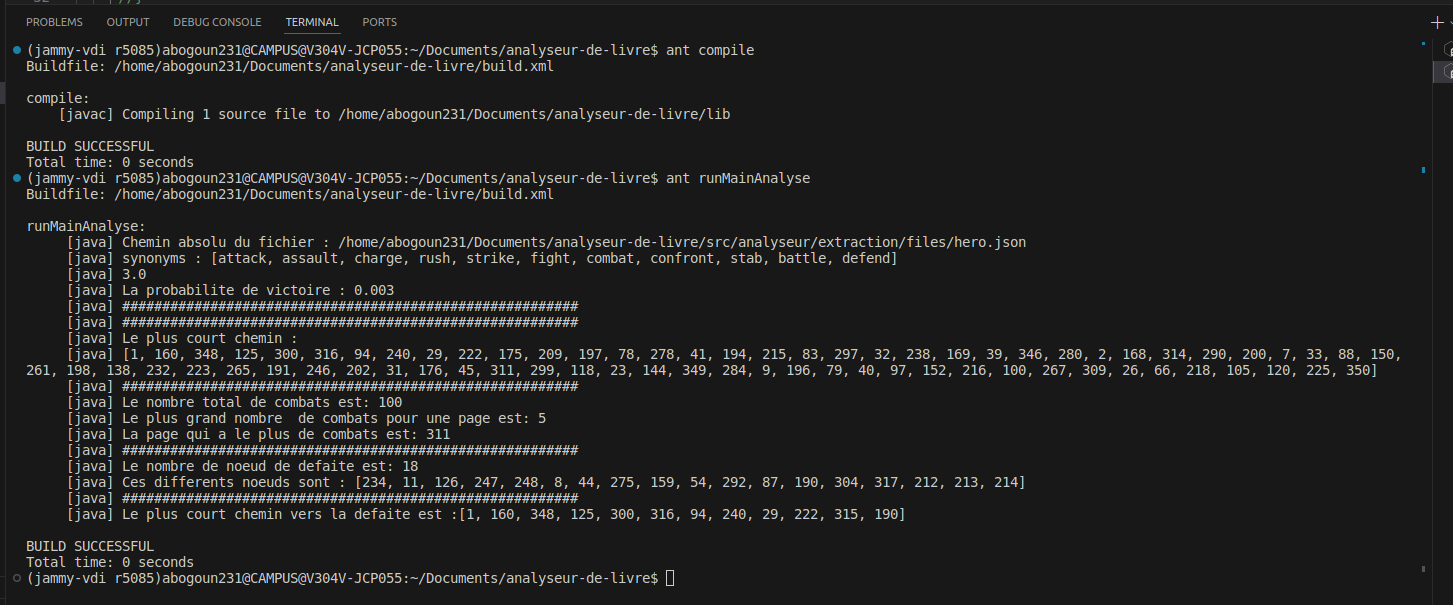
\includegraphics[width=16cm,height=16cm]{images/MainAnalyse.png}

\section{Les difficultés rencontrés}
\subsection{Difficultés rencontrées pour l'extraction des pages dans un fichier texte}
Ici,la difficulté a été de pouvoir récupérer les données dans un fichier texte quelconque. De trouver la bonne manière de procéder enfin d'extraire les informations requise.

\subsection{Difficultés rencontrées lors de la recherche du plus court chemin vers la victoire}
Au début je me suis retrouvé confronter au problème de référence sur les objets nodes qui constituaient mon graphe car mon algorithme fonctionnait sur le fait de partir d'un nœud pour accéder au nœud suivant et lui aussi à son nœud suivant et ainsi de suite, mais les nœuds qui constituaient la liste d'adjacente de mon nœud en court, je ne parvenais pas à accéder à leurs listes d'adjacente car même si ces nœuds dans ma liste d'adjacente portaient le même nom que les vrais nœuds du graphe, ils n'avaient pas les mêmes références, ce qui faisait que ces nœuds ci n'avaient pas d’éléments dans leur liste d'adjacente contrairement aux vrais nœuds de mon graphe et ça m'a pris énormément de temps avant de trouver une solution à ce problème de référence.

\subsection{Difficultés rencontrées lors de la recherche de tous les chemins qui nous mène à la victoire}
J'ai rencontré des difficultés en essayant d'appliquer l'algorithme de DAG Directed Acyclic Graph (Graphe Orienté Acyclique) au début de mon travail de recherche. Cependant, j'ai réalisé que résoudre la solution prenait trop de temps.
J'ai également essayé d'utiliser l'algorithme de tri topologique en explorant diverses méthodes. Malgré mes efforts, l'utilisation de cet algorithme a donné lieu à l'affichage d'une liste vide, ce qui m'a obligé à réévaluer ma stratégie de résolution.

\section{Les solutions trouvées}
\subsection{La solution trouvée pour l'extraction dans un fichier texte}
Dans un premier temps, nous avons utilisé une expression régulière pour récupérer chaque page du
livre et le stocker dans un tableau. Puis parcourir ce même tableau et extraire les données dans 
chaque page du livre.

\subsection{La solution trouvée pour la recherche du plus court chemin vers la victoire}
J'ai demandé à la partie modèle de me fournir une map possédant comme clé l'id du nœud, grâce à ça une fois arriver aux nœuds de la liste d’adjacent, il me suffisait de récupérer leur id et de récupérer le vrai nœud possédant cet id car lui à son tour grâce à sa liste d'adjacent me permettait de poursuivre comme il faut l'exécution de mon algorithme ainsi trouver le plus court chemin vers la victoire.

\subsection{La solution trouvée pour la recherche de tous les chemins qui nous mène à la }
Face à cette question, j'ai choisi d'utiliser l'algorithme BFS Breadth-First Search (parcours en largeur d'abord), qui s'est avéré être une alternative plus efficace et plus rapide pour trouver tous les chemins souhaités.

La transition vers l'algorithme BFS m'a permis de surmonter les difficultés initiales et d'avancer considérablement dans la résolution du problème de recherche de chemins.
J'ai pu obtenir des résultats plus rapidement en utilisant l'algorithme BFS, ce qui a contribué à l'avancement de mon travail de recherche.


\section{Perspectives d'amélioration du projet}
    Il y a toujours des perspectives d’amélioration pour notre projet, nous pouvons pensé à l'implémentation de l'algorithme de Dijkstra afin de voir lequel est plus rapide parmi les deux et d'opter pour ça. Non seulement ça, nous pouvons revoir l'affichage de notre graphe pour avoir le même graphe à chaque fois qu'on lance le main, ne plus avoir des dispositions aléatoire des nœuds. Pour étendre notre analyse nous pouvons aussi chercher tous les chemins possible pour atteindre la victoire.
	

\section{Conclusion}
La réalisation de ce projet a été une occasion pour nous membre de ce groupe d'apprendre
encore plus le langage de programmation Java. Pendant ce projet, nous avons pu appliquer ce
que nous avions appris dans les CM, les TP de ce semestre et ceux du semestre passé à savoir :
la programmation orientée objet, la conception d'applications et d'autre savoir-faire,
d'un point de vue humain, nous avons appris à mieux travailler en équipe, à communiquer,
à bien organiser un travail d'équipe et le plus important à combler nos lacunes. Nous avons
également appris à travailler à distance en utilisant les outils de travail de groupe comme SVN.
Enfin, ce rapport a également mis en évidence plusieurs domaines potentiels de développement futur, tels que l'optimisation des algorithmes d'analyse,les algorithmes de force ainsi que l'extension de la compatibilité avec d'autres formats de livres-jeux.


\section{Bibliographie}
\nocite{*}
\bibliographystyle{unsrt} 
\bibliography{fichier}


\end{document}
